\chapter{Training \& Testing of the
Detector}
\label{Chapter 5}
In this chapter we are going to discuss the training and testing of a detector. Detection is a process to identify and localize the object within an image besides classification i.e. where and what are the objects present in an image. Many states of the algorithms exist for detection including RCNN, Fast RCNN, Faster RCNN, YOLO and SSD etc. Among them YOLO is considered as extremely faster and accurate as well. Before discussing training and testing of a detector, YOLO  is explained in detail.
\section{You Only Look Once (YOLO)}
YOLO is a real time, art of the state objection detection algorithm. Unlike other object detection algorithms that uses the region based and sliding window techniques, YOLO reads the whole image once during training and testing making it extremely fast as compared to other algorithms. The whole image is divided into total of $S \times S$ grids and $N$ bounding boxes are predicted by the model. Each bounding box is associated with the probability of the object it has detected. In this way, bounding boxes with less probability of having the required object are removed and we get a single box in the end from the remaining bounding boxes with the most shaded area as shown in figure \ref{fig:5.1}.

The first version i.e. YOLO v1 has 24 convolutional layers and 2 fully connected layers. One of the major disadvantages of this version is its disability to detect very small objects \cite{chap_5_article:1}. So, a 30 layered YOLO v2 version was introduced after some time and  layers of batch normalization were introduced after every convolutional layer in this model. The fully connected layers were removed and anchor boxes to enable multiple detection in an image were introduced \cite{chap_5_article:2}. In case there lies more than one objects to be detected in the same grid cell, then these anchor boxes help the grid cells to detect multiple objects. After two years, the third version is introduced that takes us to YOLO v3 which we are using in this project.
\begin{figure}[H]
    \centering
    \captionsetup{justification = centering}
    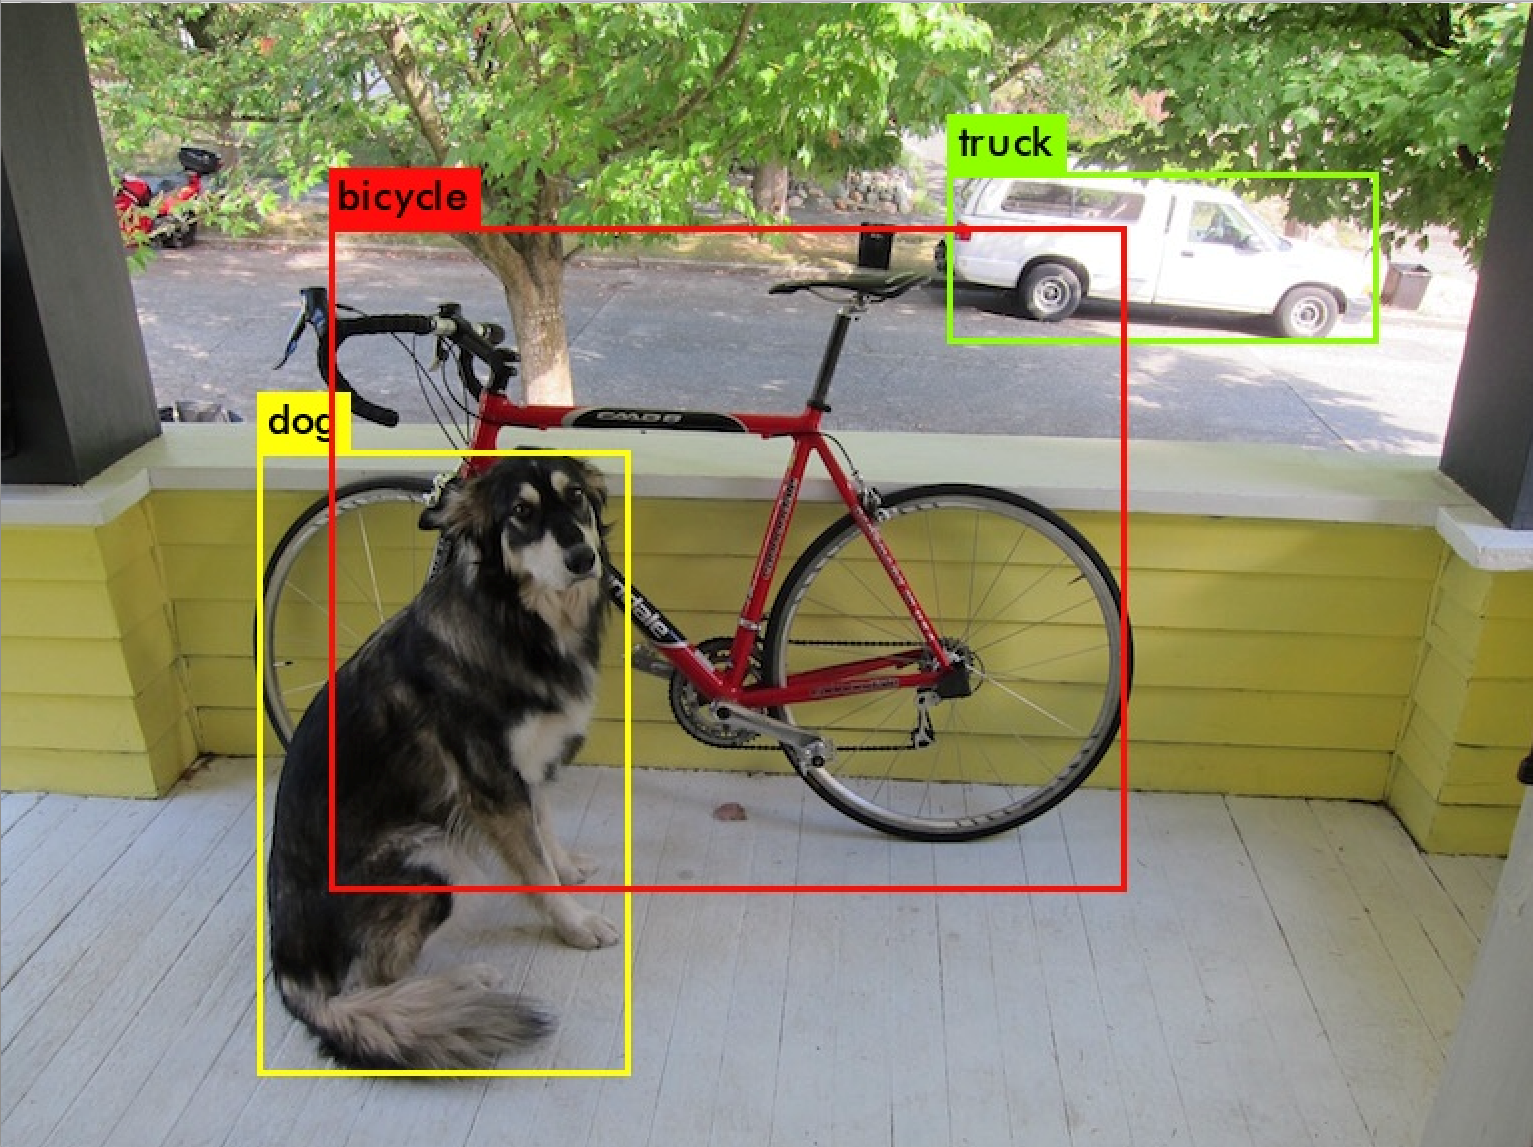
\includegraphics[scale= 0.25]{CHAPTERS/Chapter-5/images/5.1.png}
    \caption{Localization and Classification of different objects in an image } 
    \label{fig:5.1}
  \end{figure}
  \subsection{YOLO v3}
  It is latest version of YOLO with lot of improvements over the previous networks. It is considered to be three times faster than SSD giving the same accuracy. To understand the working, whole model can be split into two parts i.e. feature extractor and detector. YOLO v3 has total of 53 convolutional layers in feature extractor part also known as Darknet-53. The image firstly goes through the feature extractor. As a result, feature maps at three different scales are obtained. These features are then fed to branches of detector and we get the final output in the form of class information and bounding boxes as shown in figure \ref{fig:5.2} \cite{chap_5_article:3}.
  \begin{figure}[H]
    \centering
    \captionsetup{justification = centering}
    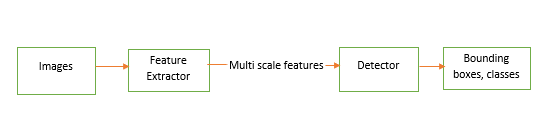
\includegraphics[scale= 1]{CHAPTERS/Chapter-5/images/5.2.png}
    \caption{Working of YOLO v3 } 
    \label{fig:5.2}
  \end{figure}
  \subsubsection{Darknet53}
    It has total of 53 convolutional layers in the feature extractor part also known as darknet-53 and its architecture is shown in figure \ref{fig:5.3}. The whole architecture of darknet-53 can be thought of as multiple blocks of two convolutional layers. These blocks are usually known as residual blocks. Convolutional layers of stride 2 are used in between these blocks that reduce the size of feature maps as shown in \ref{fig:5.3} As YOLO v3 is a multi-scale detector, feature maps from the last three residual blocks will be used and fed to the next stage. The output feature vectors will be of dimensions 52$\times$52, 26$\times$26 and 13$\times$13 if we assume the image size to be 416$\times$416. However, the output feature map size can vary depending on the input image size.
\subsubsection{Multi-scale Detector}
  Now, unlike classification detection head is introduced after the feature extractor instead of classification head. YOLO v3 is designed as multi-scaled detector so that outputs of last three residual blocks are used in the detection part. Now these three feature outputs from the darknet-53 are fed into the three branches of detector consisting of multiple 1x1 and 3x3 convolutional layers before arriving at final 1$\times$1 conv layer. Thus, the output vectors will be of the shape ((52 x$\times$52 $\times$ 3 $\times$ (4+1+number of classes)),  ((26 $\times$ 26 $\times$ 3 $\times$ (4+1+number of classes)), ((13 $\times$ 13 $\times$ 3 $\times$ (4+1+number of classes)). Now, to learn what these vector means we have to understand the concept of anchor boxes.
  \begin{figure}[H]
    \centering
    \captionsetup{justification = centering}
    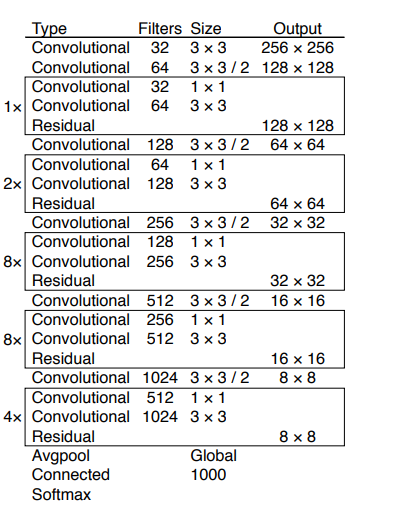
\includegraphics[scale= 1]{CHAPTERS/Chapter-5/images/5.3.PNG}
    \caption{Architecture of Darknet-53} 
    \label{fig:5.3}
  \end{figure}
\subsubsection{Anchor Boxes}
Anchor boxes are predefined aspect ratios which are determined by running K-means on the whole dataset before training. Now these anchor boxes are allotted to all of the grid cells sharing the same centroid. Then we determine which anchor box overlap with the ground truth box and decide the one which has highest value of IoU. Intersection over union (IoU) is defined as the ratio of area of overlap between both boxes as shown in figure \ref{fig:5.4a} to the area of union i.e. the total area occupied by both the ground truth box and anchor box as shown in figure \ref{fig:5.4b}.
\begin{equation}
    IoU = \frac{Area of overlap}{Area of Union}
\end{equation}

  \begin{figure}[H]
  \centering
  \begin{subfigure}[t]{0.3\textwidth}
      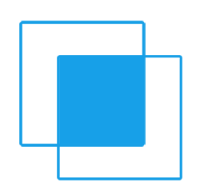
\includegraphics[scale = 0.7]{CHAPTERS/Chapter-5/images/5.4a.PNG}
      \caption{Area of overlap}
      \label{fig:5.4a}
  \end{subfigure}
  \begin{subfigure}[t]{0.3\textwidth}
      
\includegraphics[scale = 0.7]{CHAPTERS/Chapter-5/images/5.4b.PNG}
      \caption{Area of union}
      \label{fig:5.4b}
  \end{subfigure}
  \caption[]{Area of union and overlap between two bounding boxes}
  \label{fig:11.4}
\end{figure}
YOLO v3 has three anchor boxes per grid cell so there will be 52 $\times$ 52 $\times$3, 26 $\times$ 26 $\times$ 3 and 13 $\times$13 $\times$3 anchor boxes for each scale. Now for each anchor box the model has to predict three things. Firstly the 4 values to define the location of anchor box. Secondly, one value to indicate whether object is present in it or not. Thirdly, the values for probabilities  for all classes to define this anchor box belongs to which class. Thus, total number of values the model is going to predict against each anchor box becomes (4+1+number\_of\_classes). 
\subsubsection{Loss Function}
Now we have obtained the final output of detection model we can compute the loss by comparing it to the ground truth label. The total loss function in YOLO v3 is equal to the sum of four type of losses i.e. centroid loss, height and width loss, classification loss and objectness loss i.e. whether there is any object in the bounding box or not. Thus, the overall loss function can be defined by the following equation:
\begin{equation}
\begin{split}
    Loss &= (\lambda_{coord} * Sum(Mean Square Error((t_x,t_y),                 (t_x^{'},t_y^{'}))*obj mask) \\
   &+(\lambda_{coord} * Sum(Mean Square Error((t_w,t_h), (t_w^{'},t_h^{'}))*obj mask) ) \\
   &+ Sum(Binary Cross Entropy(obj, obj^{’}) * obj mask)\\
   &+ \lambda_{noobj} * Sum(Binary Cross Entropy(obj, obj^{’}) * (1 -obj mask)*(ignore mask) \\
   &+ Sum(Binary Cross Entropy(class, class^{’}))
\end{split}
\end{equation}

Now in the centroid loss, relative location of ground truth box centroid with respect to grid cell is represented by $t_{x}$ and $t_{y}$ while $t'_{x}$ and $t'_{y}$ represents the centroid of the bounding box predicted by the detector. Thus, mean square error is used because it is a kind of regression problem. We can ignore the loss of the cells which do not contain any object by multiplying it with the $objmask$ whose value is either 1 or 0 showing that required object is present in it or not. Now to calculate the values of $t_{x}$ and $t_{y}$ we can use the following equations:
\begin{equation}
    b_x = sigmoid(t_x) + C_x
\end{equation}
\begin{equation}
    b_y = sigmoid(t_y) + C_y
\end{equation}

In these equations bx and by denotes the absolute values of the centroid locations. The $t_{x}$ and $t_{y}$ are the centroid location with respect to the top left corner of the grid cell. That is why we need to add $C_{x}$ and $C_{y}$ which represent the absolute top left position of grid cell. In this way original ground truth label can be simply converted into the required target labels by inverting the formula to find out $t_{x}$ and $t_{y}$from $b_{x}$ and $b_{y}$ respectively. Similarly, in case of  width and height loss $t_w$ and $t_h$ can be found out from the absolute values of width $b_w$ and height $b_h$ respectively using the following equations:
\begin{equation}
    b_w = exp(t_w) + p_w
\end{equation}
\begin{equation}
    b_y = exp(t_h) + p_h
\end{equation}
In the third part of equation, binary cross-entropy is used to find out whether the required object is present in the cell or not rather than mean square error which was used in YOLO v2. Now, we do not want to network to cheat us by proposing objects everywhere. That is why non-object loss is used to compensate these false positive claims. $\lambda_{noobj}$ is taken equal to 0.5 to make sure the model is not dominated by the cells that does not contain objects. Lastly, Binary cross-entropy is used to determine the classification loss.
  \begin{figure}[H]
    \centering
    \captionsetup{justification = centering}
    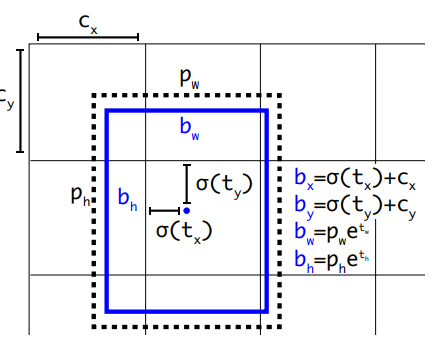
\includegraphics[scale= 0.7]{CHAPTERS/Chapter-5/images/5.5.PNG}
    \caption{Absolute and Relative dimensions of a bounding box} 
    \label{fig:5.5}
  \end{figure}
  
  \section{Preparation of Dataset}
  \subsection{Collection of Data}
  A deep learning  detection algorithm requires a set of examples labelled images from which it can learn to localize and classify the objects present within an image. We are going to detect four classes of vehicles i.e. Bus, Car, Truck and Motorcycle in this project. There are total of 4000 images with 1000 images of each class. Most of the images are downloaded from the Google Open Images V6 using the OIDv4 toolkit. It contains approximately 16 M bounding boxes on almost 1.9 M diverse images for 600 different classes. Moreover, some of the images are taken from the dataset used in classification. We can plot some of the images from the dataset to have a look at them using the python script given in listing \ref{listing:10}. The plot of the images is shown in figure \ref{fig:5.6}
\linespread{1.0}
\begin{longlisting}
\begin{minted}[bgcolor=bg,
    frame = lines,
    framesep = 2mm]{python}
import matplotlib.pyplot as plt
from matplotlib.image import imread
path = './images/'
f=plt.figure()
for i in range(1,10):
    f.add_subplot(3,3,i)
    filename = path + str(i) + '.jpg'
    image = imread(filename)
    plt.imshow(image)   
    f.show()
\end{minted}
\caption{Python script to plot some images from the dataset}
\label{listing:10}
\end{longlisting}
\begin{figure}[H]
\centering
\captionsetup{justification = centering}
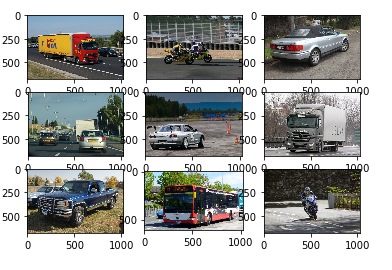
\includegraphics[scale= 1]{CHAPTERS/Chapter-5/images/5.6.PNG}
 \caption{Plot of some images from the dataset } 
 \label{fig:5.6}
 \end{figure}
 \subsection{Labelling of Images}
 In order to learn from images, the detection model needs to know where and what are the objects present in all the images. For this purpose, we need to draw bounding box around all the objects present in the dataset and label them accordingly. The images downloaded from Google Open Images V6 are already labelled so their annotation files are downloaded alongside the images. However, all the other images downloaded from other sources need to be annotated. We used the open source labelling and annotating tool for image and video known as VoTT (Visual Object Tagging Tool). After setting up the project the bounding boxes around the images can be drawn as shown in figure \ref{fig:5.7}.
\begin{figure}[H]
\centering
\captionsetup{justification = centering}
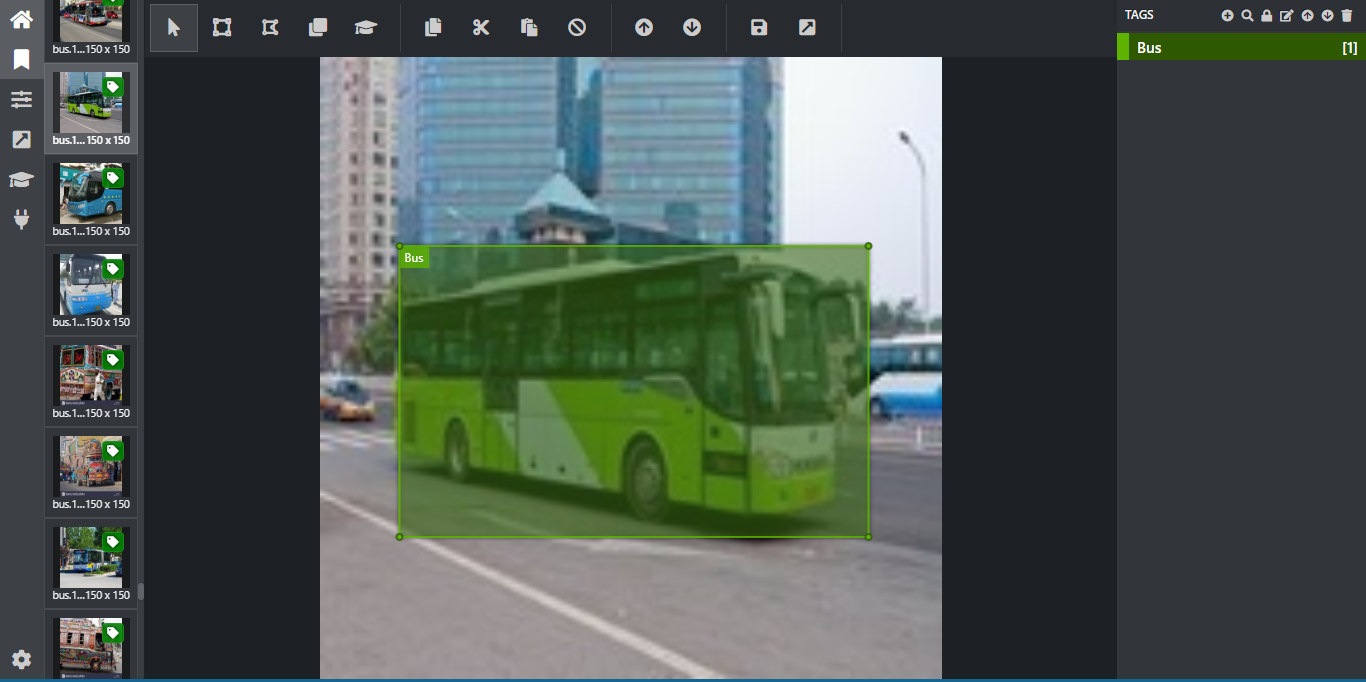
\includegraphics[scale= 0.3]{CHAPTERS/Chapter-5/images/5.7.PNG}
\caption{Labelling of images using VoTT } 
\label{fig:5.7}
\end{figure}
Once all images are labelled, all the annotations are exported into the PASCAL VOC format. All the information about labels and position of bounding boxes is stored in these xml files.
\subsubsection{Conversion of labels to YOLO v3 Format}
The YOLO v3 model does not accept the annotation files in .xml format. Thus, we need to convert the annotations to the type that YOLO accepts. YOLO v3 needs a .txt file with the information of label and coordinates of bounding boxes. So, these annotation files in .xml format are converted into YOLO v3 format using a python script. 

The output .txt files has label information in the first column in the form 0,1,2,3 depending upon the number of classes and the remaining columns contain the normalized coordinates of bounding boxes as shown in the listing \ref{listing:11}

\begin{longlisting}
\begin{minted}[bgcolor=bg,
    frame = lines,
    framesep = 2mm]{python}
1 0.2053125 0.6865051478770132 0.140625 0.20919299999999993
1 0.84125 0.6274570248901905 0.03312499999999996 0.11538499999999982
1 0.871875 0.6146927364568081 0.0318750000000001 0.08536499999999995
\end{minted}
\caption{Annotation file in the YOLO v3 format}
\label{listing:11}
\end{longlisting}

\section{Training of Detector}
\subsection{Setting up Environment}
There are a lot of images to be processed during the training process. To process such large set of  images, high end GPU is needed. Due to unavailability of a Nvidia GPU in the system, we used Google Colab. It is an  online platform having high end GPUs free provided by Google for training up to 12 hours. Enabling a GPU in the notebook settings can accelerate the process of training. 
\subsection{Cloning and Building Darknet}
Darknet is an open source framework that is used to train neural networks. It can be used as a framework for running YOLO v3 i.e. it makes the architecture of the models. It is written in C/CUDA which makes it very fast. Firstly, we have to clone its GitHub repository in cloud using command given in listing \ref{listing:12}.
\begin{longlisting}
\begin{minted}[bgcolor=bg,
    frame = lines,
    framesep = 2mm]{python}
# clone darknet repo
!git clone https://github.com/AlexeyAB/darknet
\end{minted}
\caption{Python command to clone darknet}
\label{listing:12}
\end{longlisting}
Now, before building darknet we have to configure some line in Makefile to enable GPU and OPENCV. This can be done manually or by running the python script shown in listing \ref{listing:13} to make inline changes in the file.
\begin{longlisting}
\begin{minted}[bgcolor=bg,
    frame = lines,
    framesep = 2mm]{python}
!sed -i 's/OPENCV=0/OPENCV=1/' Makefile
!sed -i 's/GPU=0/GPU=1/' Makefile
!sed -i 's/CUDNN=0/CUDNN=1/' Makefile
\end{minted}
\caption{Python script to enable Open CV and GPU}
\label{listing:13}
\end{longlisting}
Now we can build the darknet model using the command given is listing \ref{listing:14}
\begin{longlisting}
\begin{minted}[bgcolor=bg,
    frame = lines,
    framesep = 2mm]{python}
# make darknet (build)
!make
\end{minted}
\caption{Python command to build darknet}
\label{listing:14}
\end{longlisting}

\subsection{Downloading pre-trained weights for transfer learning}
Just as what human beings learn while doing one task can be utilized in solving the related problems. In most of the cases, human beings do not learn everything from scratch. We use and transfer a little bit of knowledge we have learned already from doing other related tasks. Similarly, transfer learning is a technique in which model is developed for one task and then way used as a starting point for another task. In other words, we can use the weights of the model trained on the one dataset as starting point in training the model to detect the objects we want. It makes the training process faster and more accurate comparatively. In this project, we are going to download pre-trained weights for the convolutional layer to make our model more accurate and converge faster. This pre-trained weight file can be downloaded in the cloud using the command given in \ref{listing:15}
\begin{longlisting}
\begin{minted}[bgcolor=bg,
    frame = lines,
    framesep = 2mm]{python}
# upload pre-trained convolutional layer weights
!wget http://pjreddie.com/media/files/darknet53.conv.74
\end{minted}
\caption{Python command to download pretrained weights for convolutional network}
\label{listing:15}
\end{longlisting}
\subsection{Configuring Files for training}
\subsubsection{Custom config file}
There a comes a configuration file for training the detector with the darknet. This file needs to be configured according to the requirement. Firstly, set the batch size and subdivisions equal to 64 and 16 respectively for training the detector. The number of classes of vehicles we are going to detect are 4 as mentioned before. The general formula to decide the number of max\_batches so that it gets enough number of iterations to complete the training process is given below:
\begin{equation} 
max batches = 2000 * number of classes
\end{equation}
So, we will set max\_batches = 8000 for classes.Now after setting maximum number of batches set steps equal to 80 and 90 percent of max batches respectively. Lastly, we need to decide the number of filters in convolutional layers. The general formula usually followed for deciding the number of filters is given below:
\begin{equation} 
Number of filters = (5 + number of classes) *3
\end{equation}
\begin{equation*} 
Number of filters= 27
\end{equation*}
\subsubsection{Generating train.txt and val.txt}
Train.txt contains paths to all the training images. This file is generated using the python script shown in listing \ref{listing:16}. Once the train.txt is generated, then we split the data into 80\% training and 20\% validation.
20\% of entries from the train.txt were selected randomly to generate val.txt file.
\begin{longlisting}
\begin{minted}[bgcolor=bg,
    frame = lines,
    framesep = 2mm]{python}
import os

image_files = []
os.chdir(os.path.join("data", "obj"))
for filename in os.listdir(os.getcwd()):
    if filename.endswith(".jpg"):
        image_files.append("data/obj/" + filename)
os.chdir("..")
with open("train.txt", "w") as outfile:
    for image in image_files:
        outfile.write(image)
        outfile.write("\n")
    outfile.close()
os.chdir("..")
\end{minted}
\caption{Python script to generate train.txt file}
\label{listing:16}
\end{longlisting}
\subsubsection{.names and .data files}
In the yolo.names files, write the name of classes in the same order they were written when the xml files were converted into YOLO v3 format because in the annotation files the classes are labelled against the value of integers i.e. 0 for Bus, 1 for Car, 2 for Truck and 3 for Motorcycle. The yolo.names file is shown in the listing \ref{listing:17}
\begin{longlisting}
\begin{minted}[bgcolor=bg,
    frame = lines,
    framesep = 2mm]{python}
Bus
Car
Truck 
Motorcycle
\end{minted}
\caption{yolo.names}
\label{listing:17}
\end{longlisting}
Similarly, yolo.data file simply contains locations of the files we are going to use while training like train.txt, val.txt, yolo.names and to the backup folder where weights of the model will be saved during the training process in case runtime is disconnected. The file is shown in listing \ref{listing:18}
\begin{longlisting}
\begin{minted}[bgcolor=bg,
    frame = lines,
    framesep = 2mm]{python}
classes =4
train = data/train.txt
valid = data/test.txt
names = data/yolo.names 
backup = /mydrive/yolov3/backup/
\end{minted}
\caption{yolo.data}
\label{listing:18}
\end{longlisting}
\subsection{Training of Model}
Now, it is time train the detector as we have done all the pre-processing on the dataset and generated the required files for configuration. The training can be initiated using the command shown in listing \ref{listing:19}. It takes path to the configuration file, yolo.data and pre trained convolutional weights.
\begin{longlisting}
\begin{minted}[bgcolor=bg,
    frame = lines,
    framesep = 2mm]{python}
!./darknet detector train data/yolo.data cfg/yolov3_custom.cfg darknet53.conv.74 
-dont_show
\end{minted}
\caption{Python Script to start the training of detector}
\label{listing:19}
\end{longlisting}
The biggest disadvantage of the Google Colab is that run time gets disconnected if your computer is idle for some time. To overcome this problem, we made a backup folder in google drive  where weights of the model are stored after every 100th iteration. In this way, we can resume the training process with the help of weights stored in backup folder in case anything happens. The output for one iteration of the training process is shown in figure \ref{fig:5.8} . To get an accurate model, training process can be stopped once the average less becomes less than 1. 

\begin{figure}[H]
\centering
\captionsetup{justification = centering}
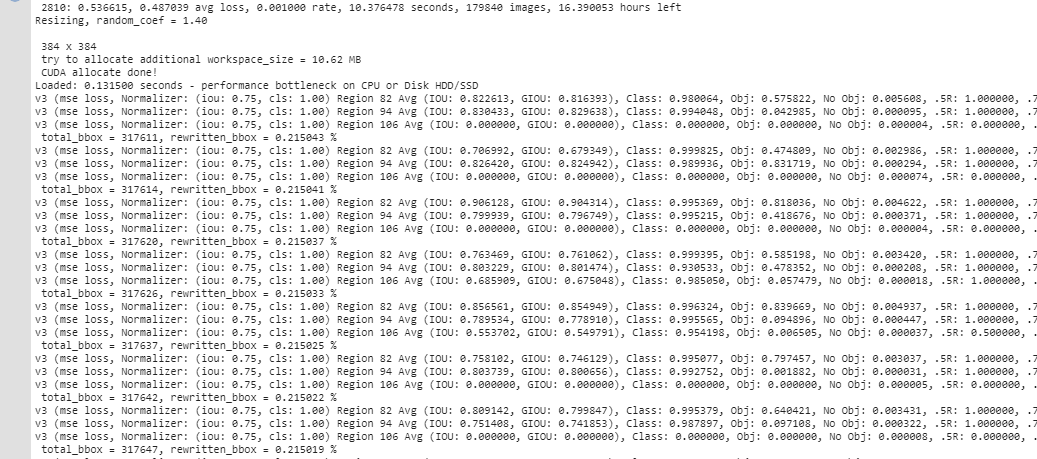
\includegraphics[scale= 0.6]{CHAPTERS/Chapter-5/images/5.8.PNG}
\caption{ Output Training log for one iteration } 
\label{fig:5.8}
\end{figure}

\section{Testing of Detector}
\subsection{Evaluation Metrices}
Before testing the detection model, we need to understand some evaluation matrices which are used to determine the performance of the detector. In case of classification it is easy to determine the accuracy of the model by simply finding out whether label predicted by the model is correct or not. However, it is not easy to evaluate the detector as we have to take into account the prediction of bounding boxes as well and whether the model detected the object or not. Most commonly metrices that are used to evaluate the detector are recall, mAP and precision. Firstly, we need to grab the concept of some commonly used terms described below to understand the evaluation metrices.
\begin{itemize}
    \item  A prediction will be True Positive if the bounding box and label predicted by the detection model is correct.
    \item A prediction will be False Positive if the predicted bounding box and label is not correct.
    \item A prediction will be False Negative if the model predicts there is no object but there is one according to the ground truth label.
\end{itemize}
\subsubsection{Precision}
Precision tells us about the number of bounding boxes predicted correctly out of total number of the predicted boxes. Ideally, its value should be 1. Mathematically, we can write:
\begin{equation}
    Precision = \frac{TP}{TP + FP}
\end{equation}
\subsubsection{Recall}
Recall tells us about the number of correctly predicted bounding boxes out of all the ground truth labels. Its value lies between 0 and 1. Mathematically, we can write:
\begin{equation}
    Recall = \frac{TP}{TP + FN}
\end{equation}
\subsubsection{Mean Average Precision}
Mean Average Precision also known as mAP is the most commonly used parameter to determine the
performance of a detector. The precision and recall are usually inversely related to each other . Increasing the threshold value usually increases the precision and decreases the recall parameter. Firstly, we need to find out the value of AP to compute mAP. Changing the value of threshold gives us a PR curve with recall on x-axis. Now, AP is can be easily computed by calculating area under the PR curve. Once it is calculated, mean Average Precision (mAP) can be found out by taking the mean value of AP over all classes we want our model to detect.
\subsection{Testing the Model}
The graph of loss and mAP for the validation data was plotted against the number of iterations during the training process. The plot is shown in figure \ref{fig:5.9}. The training process was stopped when the loss is under 1 and there is no larger variation in the value of mean Average position.
\begin{figure}[H]
\centering
\captionsetup{justification = centering}
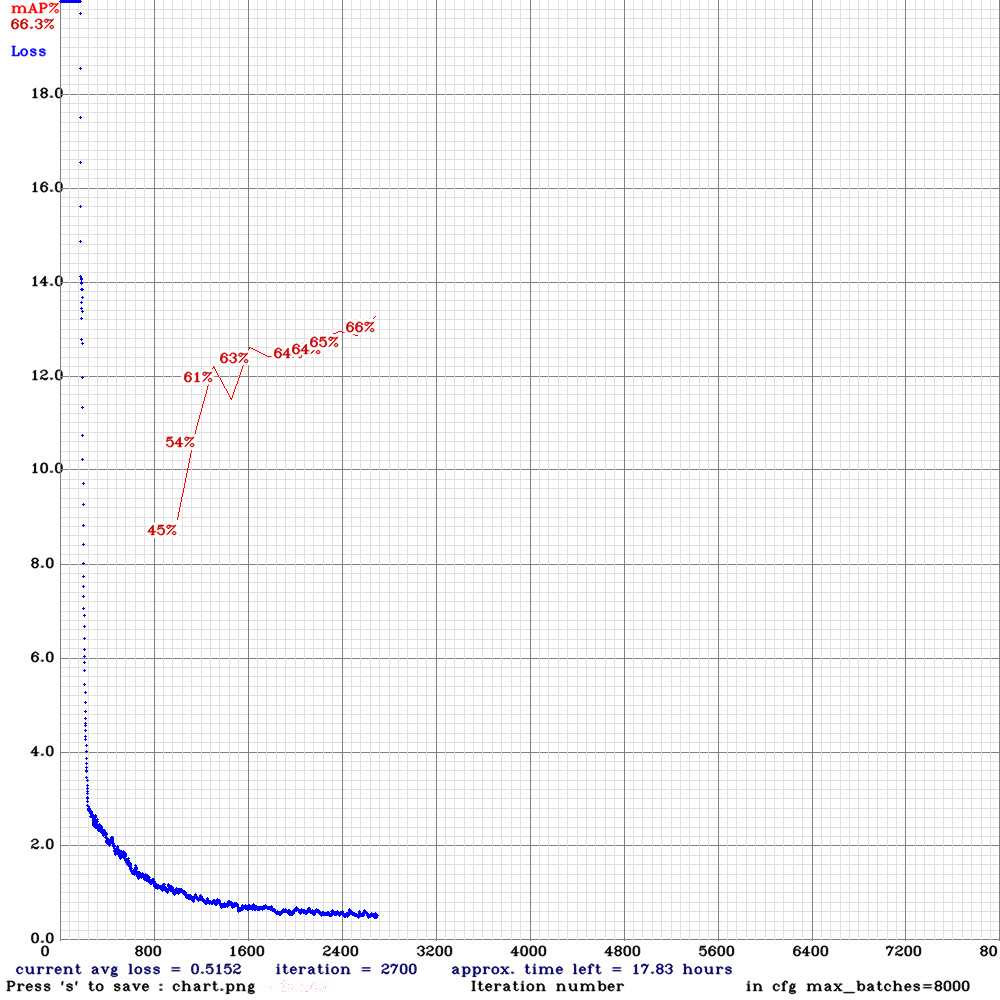
\includegraphics[scale= 0.2]{CHAPTERS/Chapter-5/images/5.9.PNG}
\caption{Plot of loss and mAP for validation data vs number of iterations}
\label{fig:5.9}
\end{figure}

Now to determine the other evaluation parameters like precision and recall, the python command shown in listing \ref{listing:20} is used firstly on the training data and the results obtained are shown in figure \ref{fig:5.10}. It can be seen that precision comes out to be 90\% at the threshold value of 0.4. Increasing the value of threshold increases the precision but the value of recall parameter is decreased. Thus, we have to find a midway between them. After trying various values of threshold, we came to the conclusion that 40\% threshold value gives the optimal value of both precision and recall. The value of mAP is also shown in the \ref{fig:5.10} that comes out to be 66\%.
\begin{longlisting}
\begin{minted}[bgcolor=bg,
    frame = lines,
    framesep = 2mm]{python}
!./darknet detector map data/obj.data cfg/yolov3_custom.cfg 
/mydrive/yolov3/backup/yolov3_custom_best.weights -thresh 0.4
\end{minted}
\caption{Python Script to determine the evaluation metrices}
\label{listing:20}
\end{longlisting}

\begin{figure}[H]
\centering
\captionsetup{justification = centering}
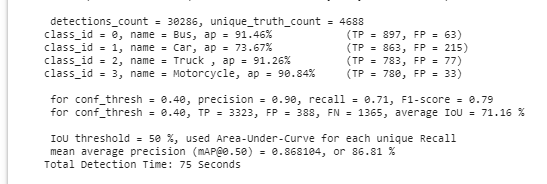
\includegraphics[scale= 0.8]{CHAPTERS/Chapter-5/images/5.10.PNG}
\caption{Evaluation Metrices for training data at threshold value of 0.4}
\label{fig:5.10}
\end{figure}
Similarly, the evaluation metrices are determined for the test data and the output results are shown in figure \ref{fig:5.11}. The precision comes out to be 82\% and is less than training data. However, it is obvious for detector to give less precision than the training data because it has not seen the testing data before. 
\begin{figure}[H]
\centering
\captionsetup{justification = centering}
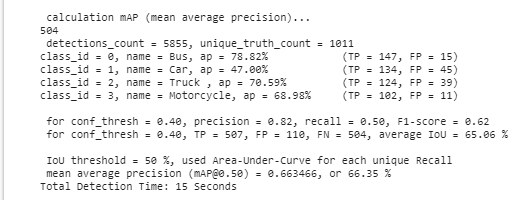
\includegraphics[scale= 0.8]{CHAPTERS/Chapter-5/images/5.11.PNG}
\caption{Evaluation Metrices for testing data at threshold value of 0.4}
\label{fig:5.11}
\end{figure}

Now to observe the working of the detector, we have to pass images to the detector model one by one and it will localize and label the classes of vehicles in return. The latest model weights were saved in the backup folder so we will pass the location of weight file and test images 1 by 1. A labelled image will be displayed on the window after processing. The python command that is used to detect the images is shown in listing \ref{listing:21} and the output images are shown in figure \ref{fig:5.12}.
\begin{longlisting}
\begin{minted}[bgcolor=bg,
    frame = lines,
    framesep = 2mm]{python}
!./darknet detector test data/obj.data cfg/yolov3_custom.cfg/mydrive/yolov3
/backup/yolov3_custom_best.weights /mydrive/yolov3/images/t7.jpg -thresh 0.3
imShow('predictions.jpg')
\end{minted}
\caption{Python Script to detect objects in an image}
\label{listing:21}
\end{longlisting}
\begin{figure*}
    \centering
    \begin{subfigure}[t]{0.475\textwidth}
        \centering
        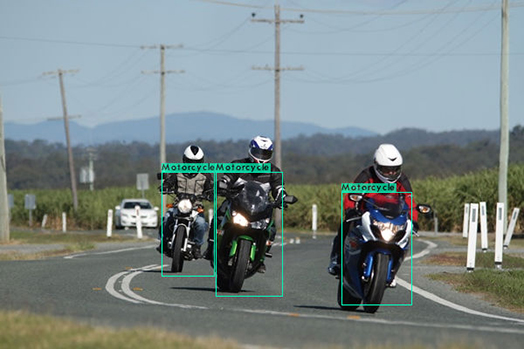
\includegraphics[width = 7cm, height = 5 cm]{CHAPTERS/Chapter-5/images/5.12a.jpg}
        \caption[]%
        {{\small }}    
        \label{fig:mean and std of net14}
    \end{subfigure}
    \hfill
    \begin{subfigure}[t]{0.475\textwidth}  
        \centering 
        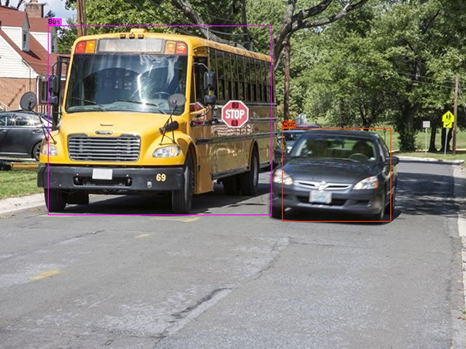
\includegraphics[width = 7cm, height = 5 cm]{CHAPTERS/Chapter-5/images/5.12b.jpg}
        \caption[]%
        {{\small }}    
        \label{fig:mean and std of net24}
    \end{subfigure}
    \vskip\baselineskip
    \begin{subfigure}[t]{0.475\textwidth}   
        \centering 
        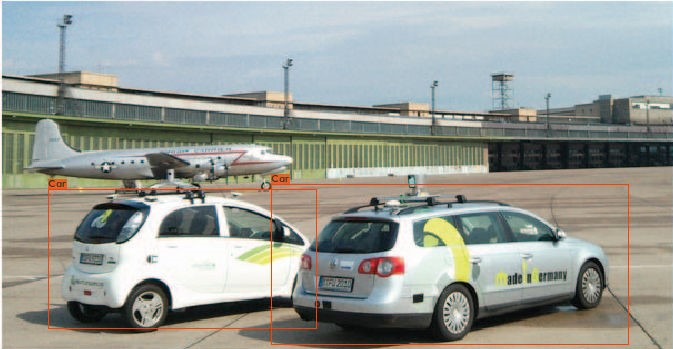
\includegraphics[width = 7cm, height = 5 cm]{CHAPTERS/Chapter-5/images/5.12c.jpg}
        \caption[]%
        {{\small }}    
        \label{fig:mean and std of net34}
    \end{subfigure}
    \quad
    \begin{subfigure}[t]{0.475\textwidth}   
        \centering 
        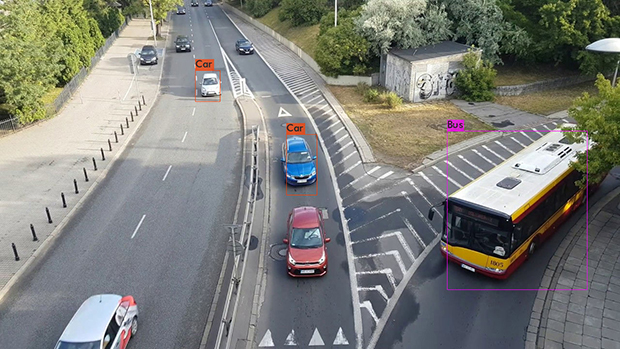
\includegraphics[width = 7cm, height = 5 cm]{CHAPTERS/Chapter-5/images/5.12d.jpg}
        \caption[]%
        {{\small }}    
        \label{fig:mean and std of net44}
    \end{subfigure}
    \caption[ ]
    {\small Output images from the Detection Model}
    \label{fig:5.12}
\end{figure*}
\section{Limitations and Future Work}
It is a well-known fact that deep learning algorithms learn better from large number of images in dataset. The deep learning model which is trained on large number of images will learn and detect images better than the one trained on smaller dataset. Although we implemented the detector model with 90\% precision, but it has certain limitations. The model does not detect all the vehicles when the image is crowded or taken from a large distance. One of the main reasons is the lack of such images in the dataset. Almost 80\% of the images in the dataset has only one or two vehicles in it. The model needs very clear pictures of vehicles to train taken at a good distance at which it can differentiate between the required classes which are not available online. Moreover, we could not train the model on more than 3000-4000 images due to the limitations of resources and time. 

In the future work, the detection model can be trained with the larger number of images to overcome its limitations. The images of the vehicles can be obtained using cameras on National Highways from the corresponding department. It will help in improving the performance of detector by increasing its precision, mAP, and other evaluation metrics. Moreover, the detection model can be used in future for detection and tracking of vehicles in automatic driving and traffic surveillance purposes.
